
\documentclass[12pt,a4paper]{article}

% -------------------------------------------------
% MCP Filesystem Server Demonstration Report
% Compile with: pdflatex mcp_filesystem_demo_report.tex
% -------------------------------------------------
\usepackage[utf8]{inputenc}
\usepackage[T1]{fontenc}
\usepackage{lmodern}
\usepackage[a4paper,margin=2.5cm]{geometry}
\usepackage{microtype}
\usepackage{graphicx}
\usepackage{xcolor}
\usepackage{hyperref}
\usepackage{listings}
\usepackage{enumitem}
\usepackage{float}
\usepackage{booktabs}
\usepackage{array}
\usepackage{caption}
\usepackage{titlesec}

% Look for images inside the screenshots folder
\graphicspath{{./Screenshots/}}

\definecolor{codebg}{RGB}{246,248,250}
\definecolor{codeframe}{RGB}{210,216,222}
\definecolor{accent}{RGB}{25,83,112}
\hypersetup{colorlinks=true,linkcolor=accent,urlcolor=accent,citecolor=accent}
\titleformat{\section}{\Large\bfseries\color{accent}}{\thesection}{0.7em}{}
\titleformat{\subsection}{\large\bfseries\color{accent}}{\thesubsection}{0.7em}{}
\setlist{itemsep=3pt,topsep=5pt}

\lstdefinestyle{terminal}{
	backgroundcolor=\color{codebg},
	frame=single,
	rulecolor=\color{codeframe},
	basicstyle=\ttfamily\small,
	breaklines=true,
	columns=fullflexible,
	keepspaces=true,
	showstringspaces=false
}
\lstdefinestyle{json}{
	backgroundcolor=\color{codebg},
	frame=single,
	rulecolor=\color{codeframe},
	basicstyle=\ttfamily\small,
	breaklines=true,
	columns=fullflexible,
	showstringspaces=false
}

% Replace the bracketed fields below before submission.
\newcommand{\StudentName}{Blada Chems Eddine }
\newcommand{\CourseName}{AI Integration}
\newcommand{\InstructorName}{Nexlevr}
\newcommand{\SubmissionDate}{\today}

\begin{document}
	
	\begin{titlepage}
		\centering
		\vspace*{2cm}
		{\Large\textsc{Practical Demonstration Report}\par}
		\vspace{1.2cm}
		{\huge\bfseries Using an MCP Filesystem Server with an AI Assistant\par}
		\vspace{0.7cm}
		{\Large Connecting Claude Desktop to local business files\par}
		\vspace{1.8cm}
		\rule{0.85\textwidth}{0.6pt}\par
		\vspace{1.2cm}
		\begin{tabular}{>{\bfseries}p{4cm}p{8cm}}
			Student: & \StudentName \\
			Course / Module: & \CourseName \\
			Instructor: & \InstructorName \\
			Submission date: & \SubmissionDate \\
		\end{tabular}
		\vfill
		\begin{minipage}{0.82\textwidth}
			\centering
			This report documents the installation and use of a Model Context Protocol (MCP) filesystem server to let an AI assistant read sample customer feedback and create a business analysis report within a restricted project directory.
		\end{minipage}
		\vspace{1cm}
	\end{titlepage}
	
	\tableofcontents
	\listoffigures
	\newpage
	
	\section{Introduction}
	
	The purpose of this practical task was to connect an AI assistant to an external tool through the Model Context Protocol (MCP), demonstrate the assistant using that tool for a realistic business activity, and explain the permissions granted.
	
	For this demonstration, Claude Desktop was connected to the Filesystem MCP server. The business scenario was to analyse a small collection of customer feedback text files and produce a Markdown report containing the main positive points, complaints, themes, and suggested improvements.
	
	\section{Tools and Environment}
	
	The following software and components were used:
	\begin{itemize}
		\item \textbf{AI application:} Claude Desktop for Windows.
		\item \textbf{MCP server:} The Filesystem MCP server package, \texttt{@modelcontextprotocol/server-filesystem}.
		\item \textbf{Runtime:} Node.js and npm/npx.
		\item \textbf{Operating system:} Microsoft Windows.
		\item \textbf{Input data:} Three sample customer feedback files.
		\item \textbf{Output:} A Markdown report named \texttt{customer\_feedback\_report.md}.
	\end{itemize}
	
	\section{MCP Server Configuration}
	
	The Filesystem MCP server was configured in Claude Desktop's configuration file. The server was launched through the Windows Node.js \texttt{npx.cmd} executable and given one permitted root directory: the project folder for this task.
	
	The effective permitted directory was:
	\begin{lstlisting}[style=terminal]
		C:\Users\chems\OneDrive\Desktop\Nexlevr\beginner\Task 2
	\end{lstlisting}
	
	The relevant server configuration was:
	\begin{lstlisting}[style=json]
		"mcpServers": {
			"filesystem": {
				"command": "C:\\Program Files\\nodejs\\npx.cmd",
				"args": [
				"-y",
				"@modelcontextprotocol/server-filesystem",
				"C:\\Users\\chems\\OneDrive\\Desktop\\Nexlevr\\beginner\\Task 2"
				]
			}
		}
	\end{lstlisting}
	
	After saving the configuration and restarting Claude Desktop, the application displayed the \texttt{filesystem} MCP server as running. The package was also tested from PowerShell and reported that it was running over standard input/output (stdio), with the same effective allowed directory.
	
	\section{Directory Structure and Test Data}
	
	The project directory was organised as follows:
	\begin{lstlisting}[style=terminal]
		Task 2/
		|-- Customer-Feedback/
		|   |-- feedback_01.txt
		|   |-- feedback_02.txt
		|   |-- feedback_03.txt
		`-- Reports/
	\end{lstlisting}
	
	The three input files contained sample feedback from customers. The \texttt{Reports} directory was initially empty. The data was used to demonstrate a simple business analysis workflow without exposing unrelated personal or business files to the MCP server.
	
	\section{Demonstration Procedure}
	
	The following task was given to Claude:
	\begin{quote}
		Use the connected filesystem tools to list the project directory, read all customer feedback files, identify positive comments and complaints, group the main themes, and create a professional Markdown report in the \texttt{Reports} folder. Work only inside the permitted project directory. Do not modify or delete the original feedback files, and do not invent customer comments or findings.
	\end{quote}
	
	Claude carried out the workflow using filesystem MCP tools. The first call to \texttt{list\_allowed\_directories} timed out. Claude retried the read-only call, and the retry succeeded. The returned allowed directory matched the configured project root.
	
	\subsection{MCP tools used}
	
	\begin{table}[H]
		\centering
		\small
		\begin{tabular}{p{0.36\textwidth}p{0.56\textwidth}}
			\toprule
			\textbf{MCP tool} & \textbf{Purpose in the demonstration} \\
			\midrule
			\texttt{list\_allowed\_directories} & Checked which directory the server permitted Claude to access. The first call timed out; the retry succeeded. \\
			\texttt{list\_directory} & Listed the contents of the project directory and later checked the output directory. \\
			\texttt{list\_directory\_with\_sizes} & Listed the customer feedback directory and its three files. \\
			\texttt{read\_multiple\_files} & Read the contents of all three feedback files. \\
			\texttt{write\_file} & Created the Markdown report in the \texttt{Reports} directory. \\
			\bottomrule
		\end{tabular}
		\caption{Filesystem MCP tools used by Claude during the task.}
	\end{table}
	
	Before writing the report, Claude checked that the \texttt{Reports} directory was empty, so the intended output filename did not already exist. It then created \texttt{customer\_feedback\_report.md}.
	
	\section{Results}
	
	The generated report summarised the three feedback files. Claude identified the following points:
	
	\begin{itemize}
		\item \textbf{Positive feedback:} Customers described the website as easy to use and attractive, found the payment process simple, and considered the prices reasonable. One customer expressed general satisfaction with the service.
		\item \textbf{Complaints:} Feedback mentioned slow delivery, slow customer-support responses, and problems using the website on a mobile device. A customer also requested real-time order tracking.
		\item \textbf{Suggested improvements:} Consider adding order tracking, reviewing delivery processes, setting a customer-support response target, and investigating the reported mobile issue.
	\end{itemize}
	
	The sample contained only three customer records. Each complaint was associated with an individual customer, so the report treated these as issues raised in the sample rather than claiming that each issue was repeatedly reported by multiple customers. The suggested improvements were presented as recommendations, not as facts stated by the customers.
	
	The output file was saved at:
	\begin{lstlisting}[style=terminal]
		Task 2\Reports\customer_feedback_report.md
	\end{lstlisting}
	
	\section{Permissions and Security Considerations}
	
	The main permission decision was to grant the filesystem server access only to the \texttt{Task 2} project directory, rather than to the user's entire computer or home directory. Claude's successful \texttt{list\_allowed\_directories} response confirmed that this was the server's effective allowed root for the demonstration.
	
	This is an example of the \textbf{principle of least privilege}: an application or tool should receive only the access needed to complete its task.
	
	Important considerations:
	\begin{itemize}
		\item The server's permitted root limits the filesystem area available through its tools.
		\item The Filesystem MCP server provides operations that can read and also write, edit, move, or delete files within its permitted area. Restricting the root does not make every operation read-only.
		\item The task prompt explicitly instructed Claude not to modify or delete the original feedback files.
		\item The input files were checked after the task and were found to remain unchanged. The report was created as a separate file.
		\item Only sample data should be used for demonstrations. Sensitive files should not be placed inside a directory granted to an MCP server unless access is necessary and authorised.
		\item Tool activity and generated files should be reviewed, especially before allowing write or other file-changing operations.
	\end{itemize}
	
	The prompt's instruction not to change the original files was an operational safeguard, not a replacement for technical access controls. The strongest protection is to grant access only to a dedicated working directory containing non-sensitive test data and to review actions that change files.
	
	\section{Verification}
	
	The demonstration was checked after Claude completed the task:
	\begin{enumerate}
		\item Claude's tool-use summary showed the filesystem MCP operations used, including directory listing, file reading, and report writing.
		\item The generated report was located in the \texttt{Reports} directory.
		\item The three original feedback files were inspected after the task and were found to be unchanged.
	\end{enumerate}
	
	No pre-task file hashes were recorded. Therefore, the unchanged-file check was a manual post-task inspection rather than a cryptographic before-and-after comparison.
	
	\section{Conclusion}
	
	The practical task successfully demonstrated how an AI assistant can use an MCP server to interact with local files for a business purpose. Claude Desktop connected to the Filesystem MCP server, confirmed the permitted project directory, read three customer feedback files, and created a Markdown analysis report.
	
	The demonstration also showed why permissions matter. Limiting the server to a dedicated project directory reduced unnecessary access, while reviewing tool calls and checking the original files helped ensure that the task was completed as intended. The exercise illustrates both the usefulness of MCP-based tool integration and the need to apply least-privilege access and human verification.
	
	\appendix
	\section{Evidence and Screenshots}
	
	The following screenshots provide visual evidence of the MCP server configuration, tool activity, generated report, and project directory.
	
	% Screenshot 1: MCP server connected
	\begin{figure}[H]
		\centering
		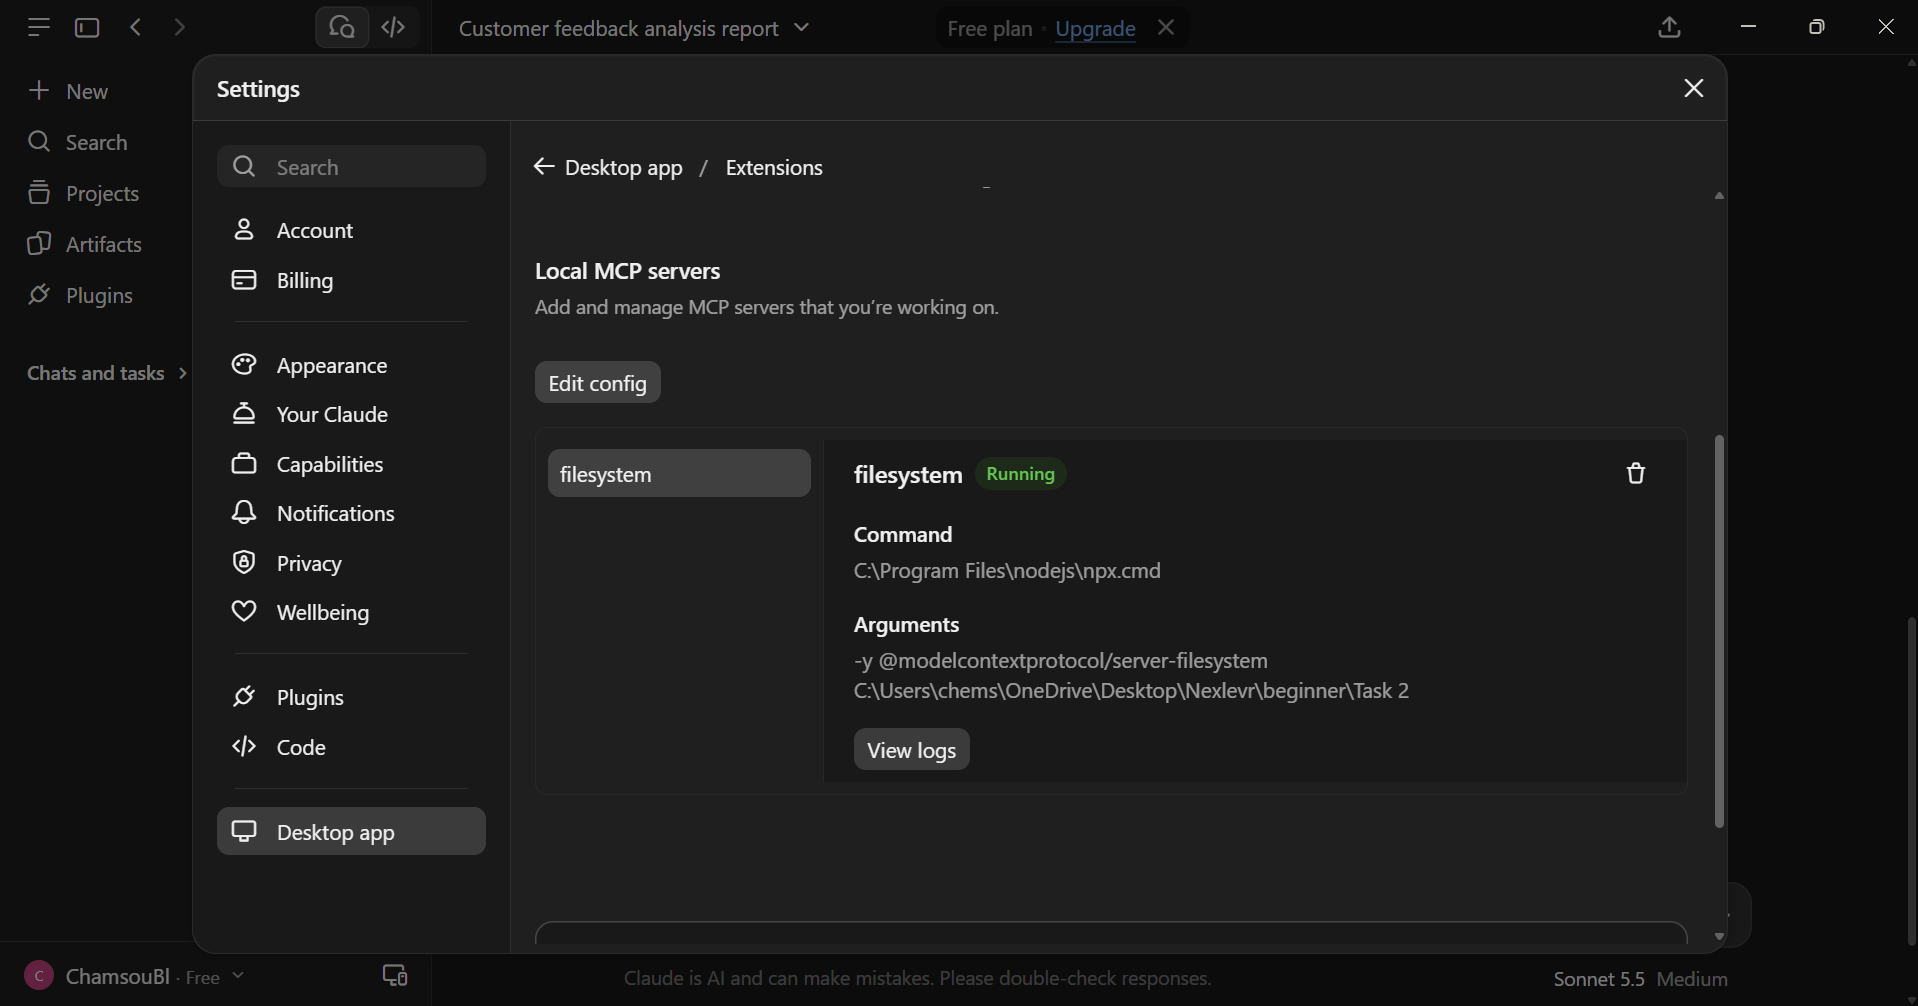
\includegraphics[width=0.9\textwidth,height=0.65\textheight,keepaspectratio]{screenshot1.png}
		\caption{Claude Desktop with the Filesystem MCP server connected.}
	\end{figure}
	
	% Screenshot 2: Allowed directory
	\begin{figure}[H]
		\centering
		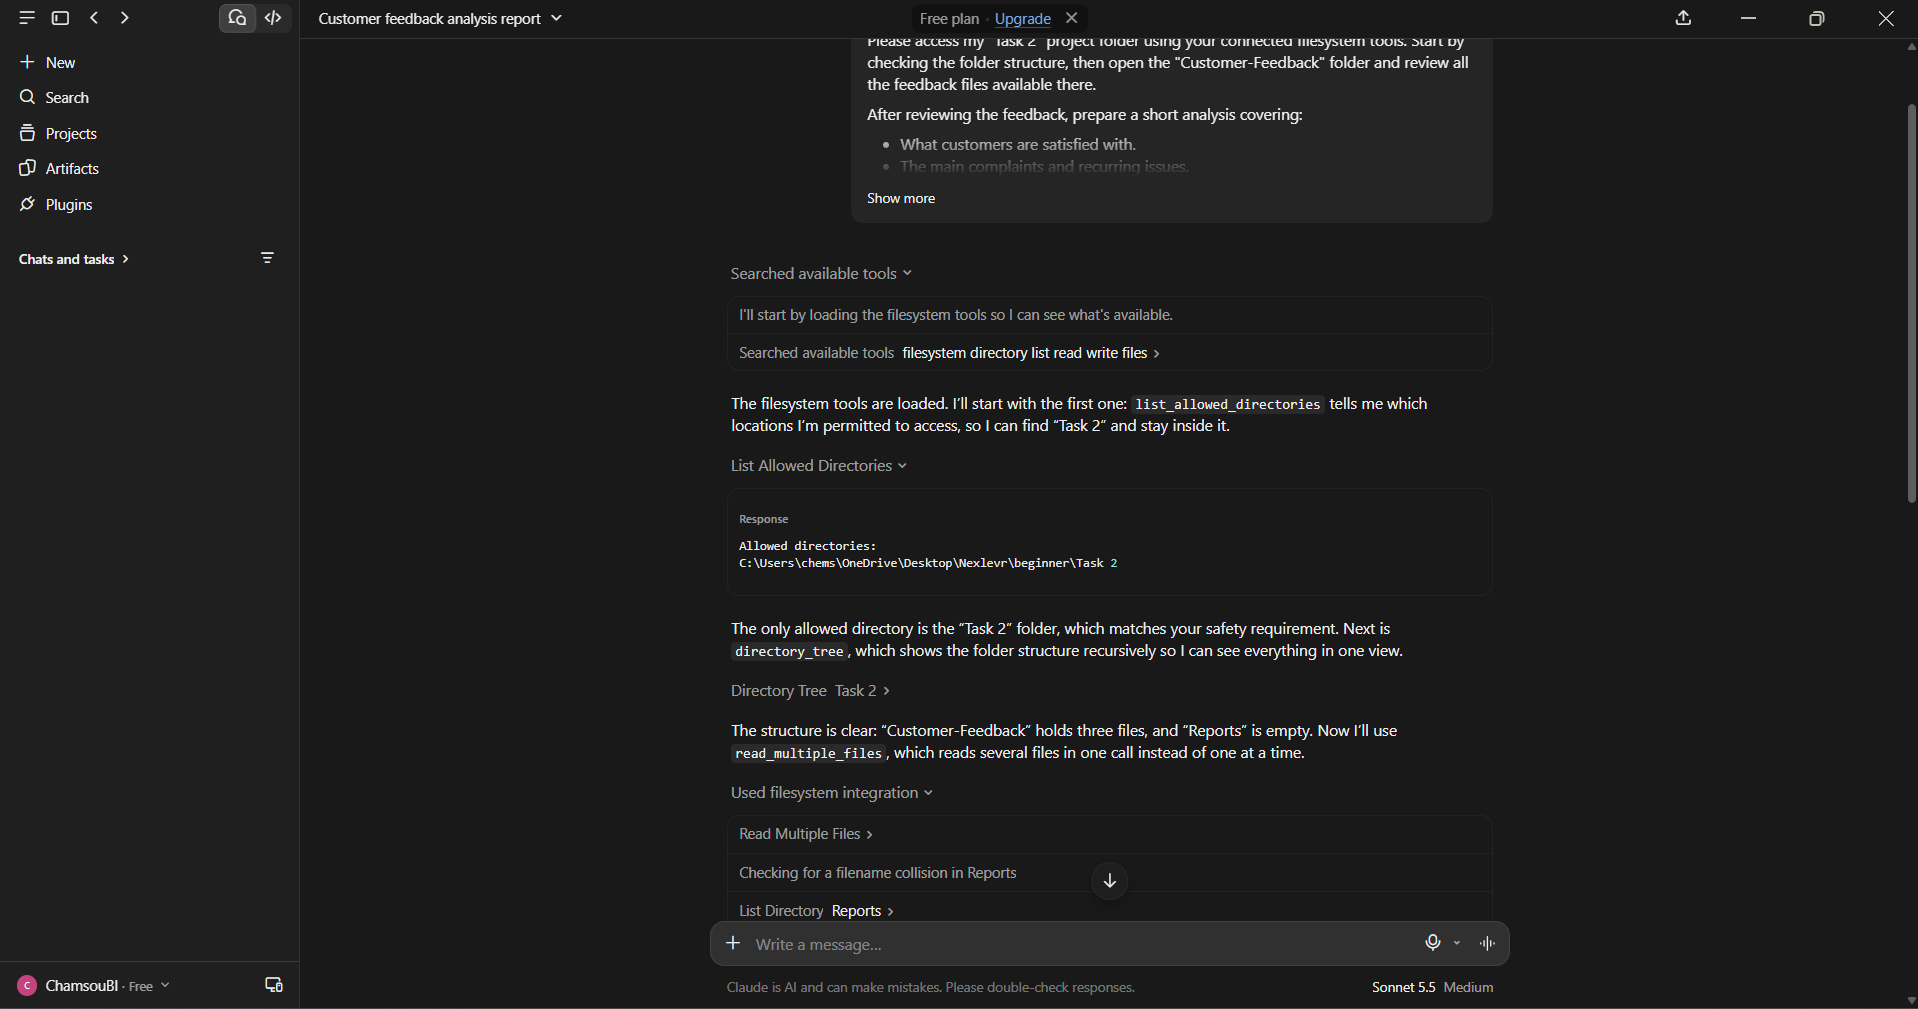
\includegraphics[width=0.9\textwidth,height=0.65\textheight,keepaspectratio]{screenshot2.png}
		\caption{The filesystem server's permitted directory.}
	\end{figure}
	
	% Screenshot 3: MCP tool activity
	\begin{figure}[H]
		\centering
		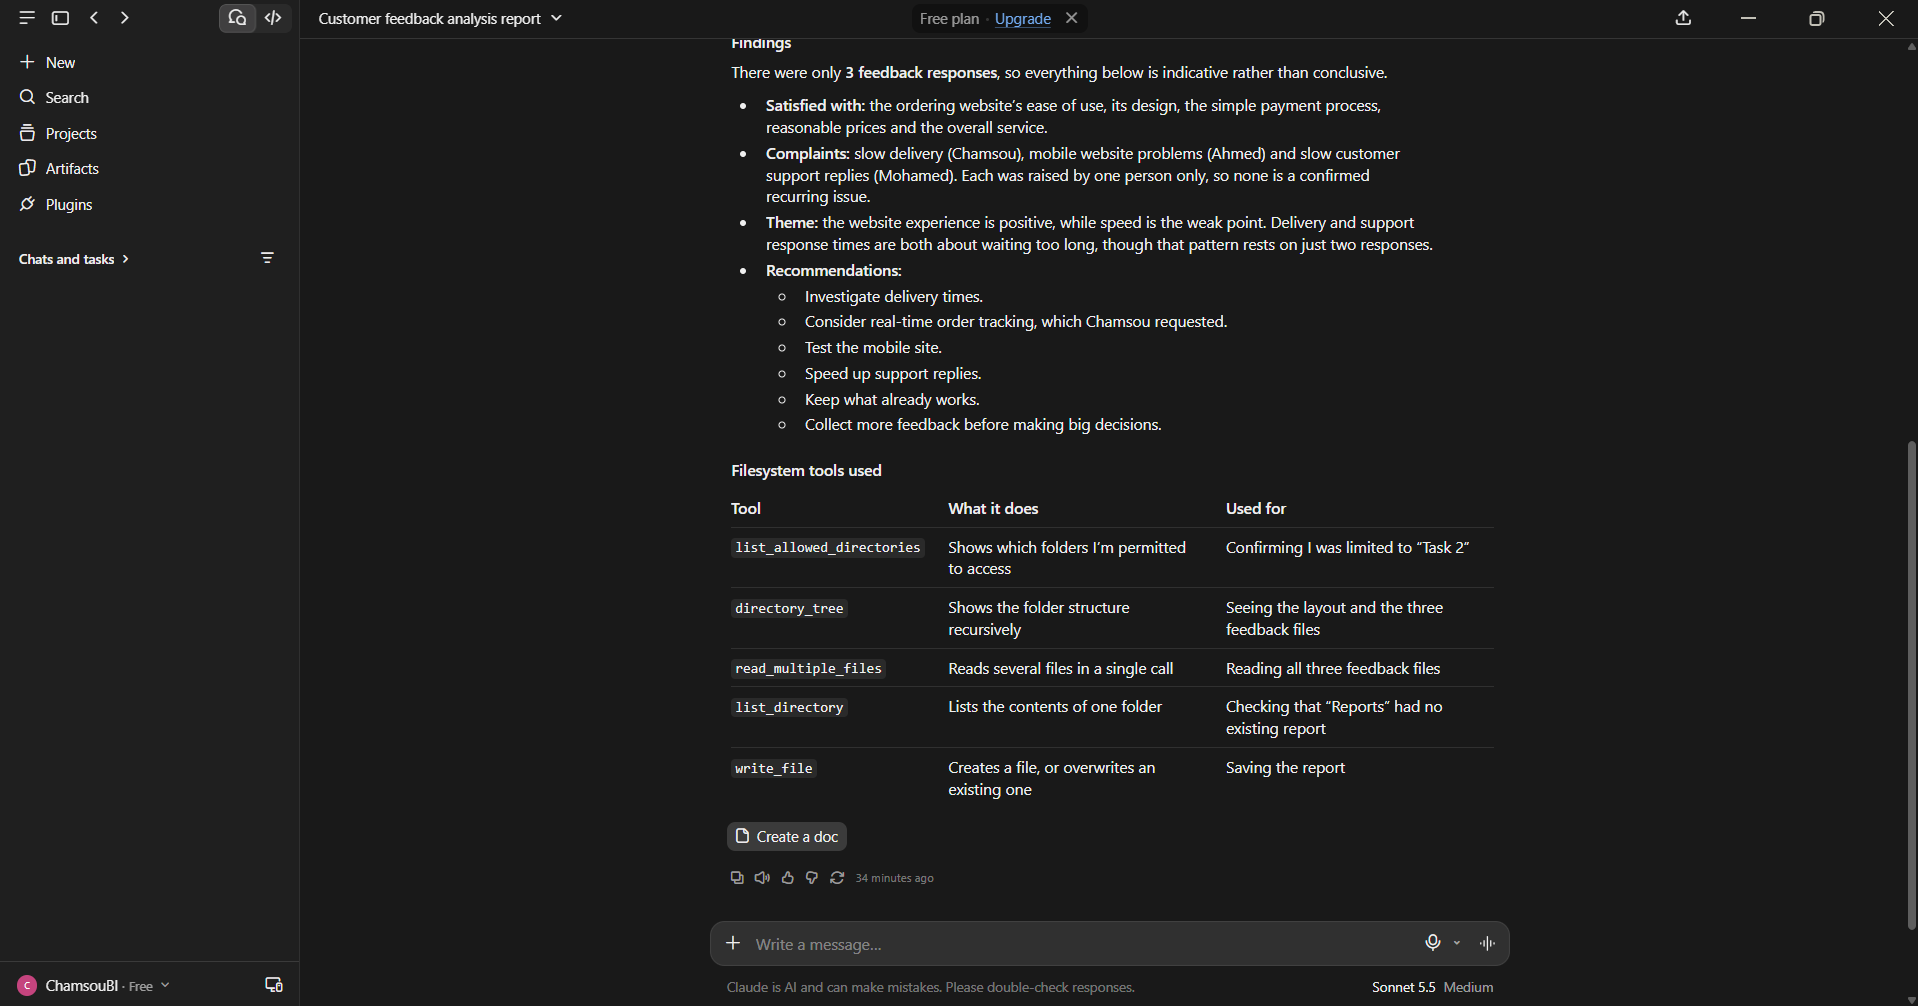
\includegraphics[width=0.9\textwidth,height=0.65\textheight,keepaspectratio]{screenshot3.png}
		\caption{Filesystem MCP tool calls during the business task.}
	\end{figure}
	
	% Screenshot 4: Generated report
	\begin{figure}[H]
		\centering
		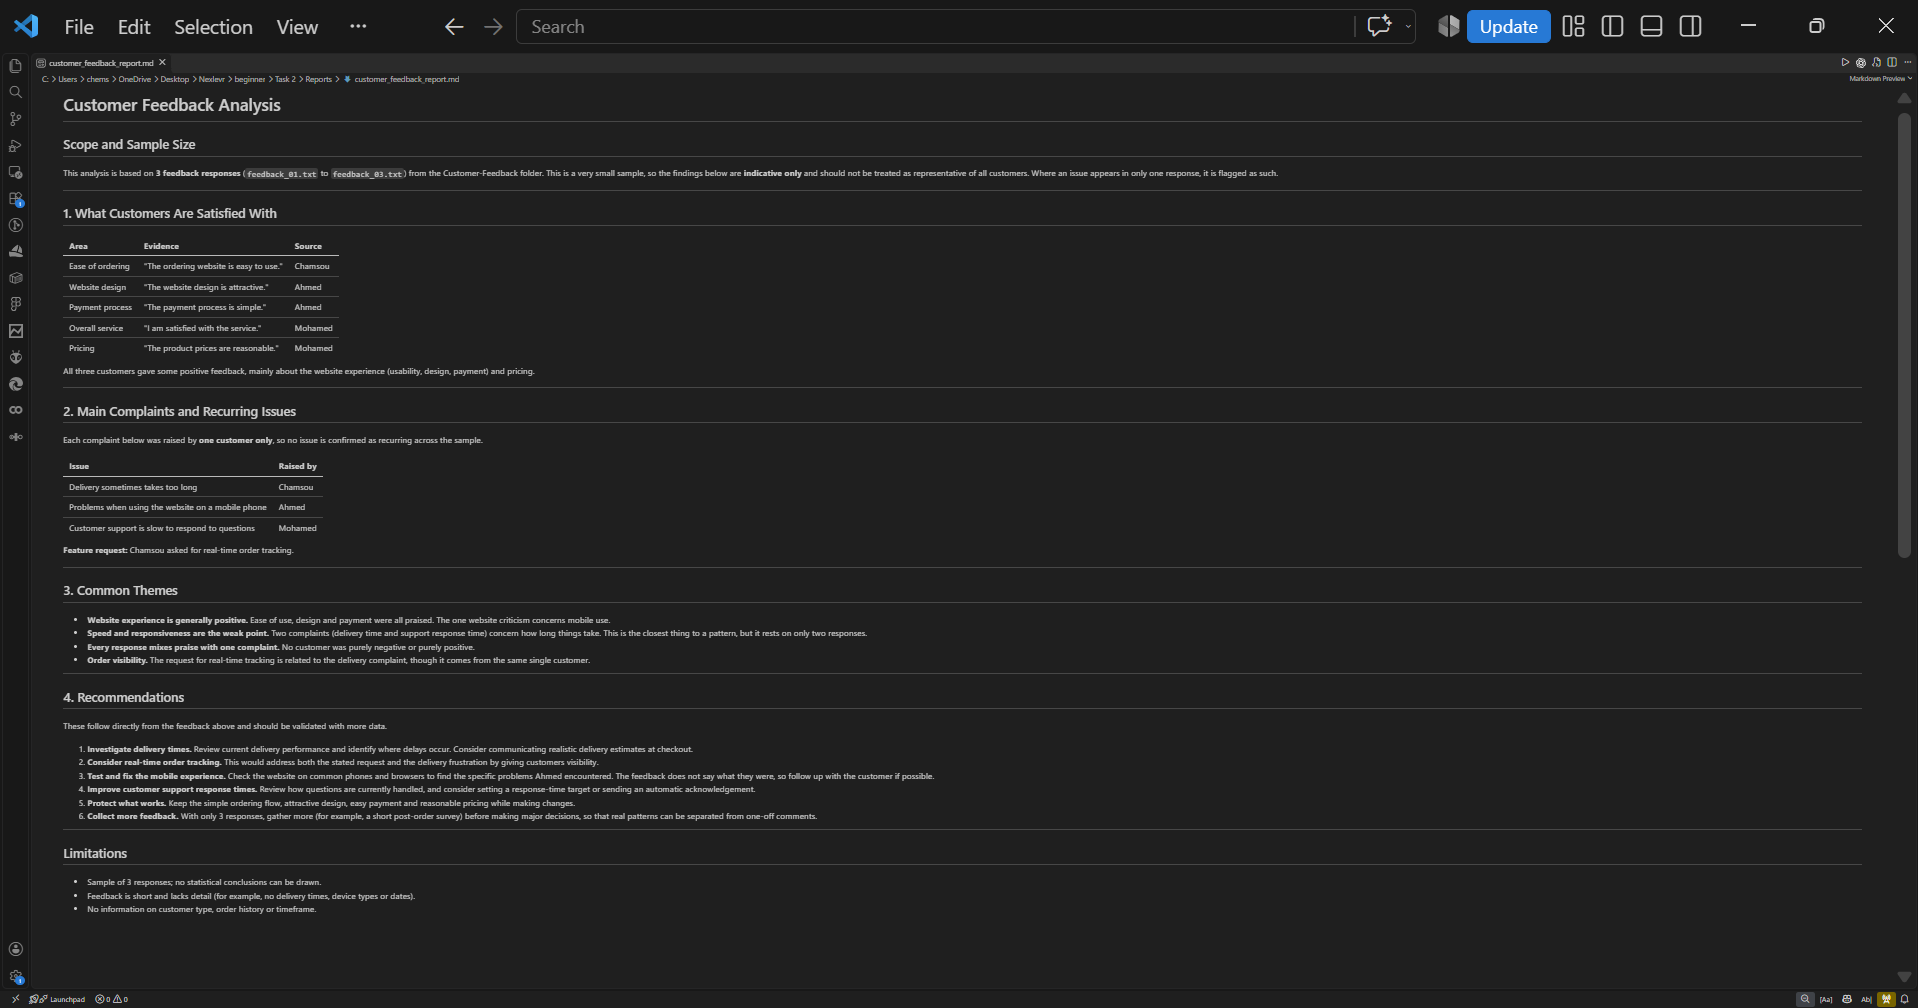
\includegraphics[width=0.9\textwidth,height=0.65\textheight,keepaspectratio]{screenshot4.png}
		\caption{The generated customer feedback analysis report.}
	\end{figure}
	
	% Screenshot 5: Project directory
	\begin{figure}[H]
		\centering
		
		\begin{minipage}{0.48\textwidth}
			\centering
			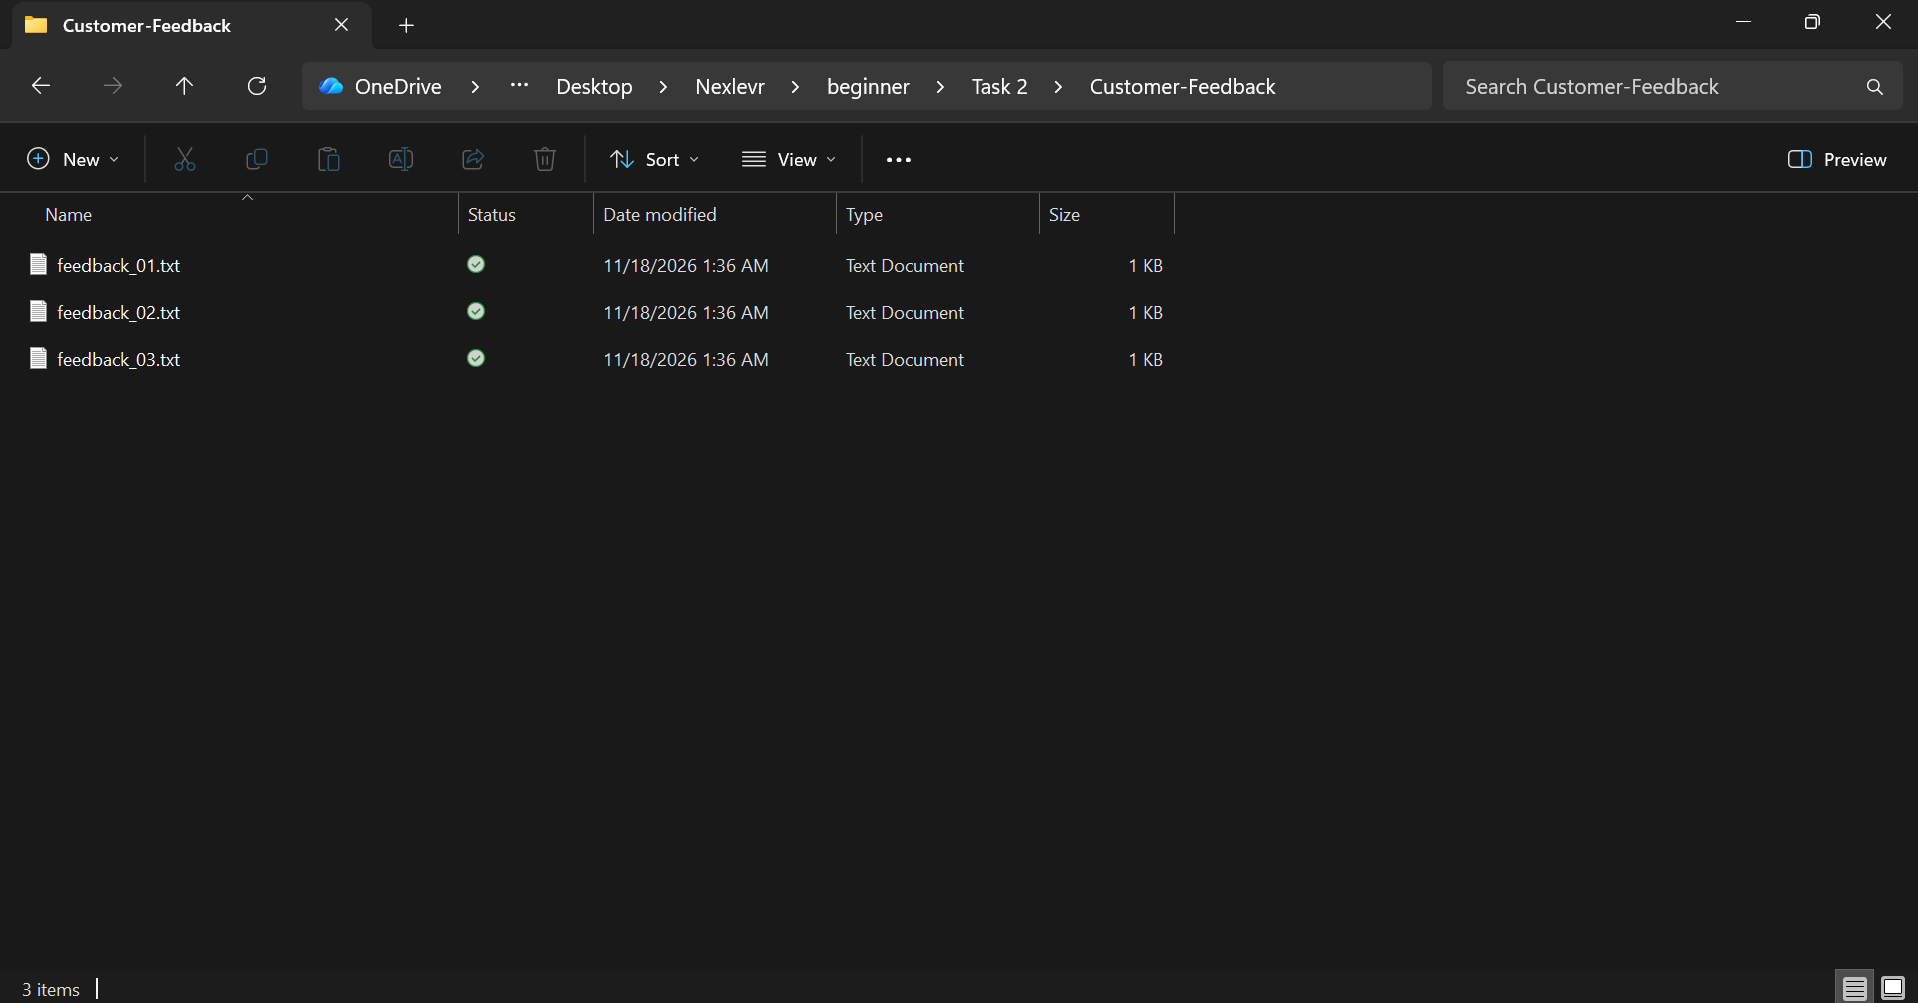
\includegraphics[width=\linewidth,height=5cm,keepaspectratio]{screenshot51.png}
		\end{minipage}
		\hfill
		\begin{minipage}{0.48\textwidth}
			\centering
			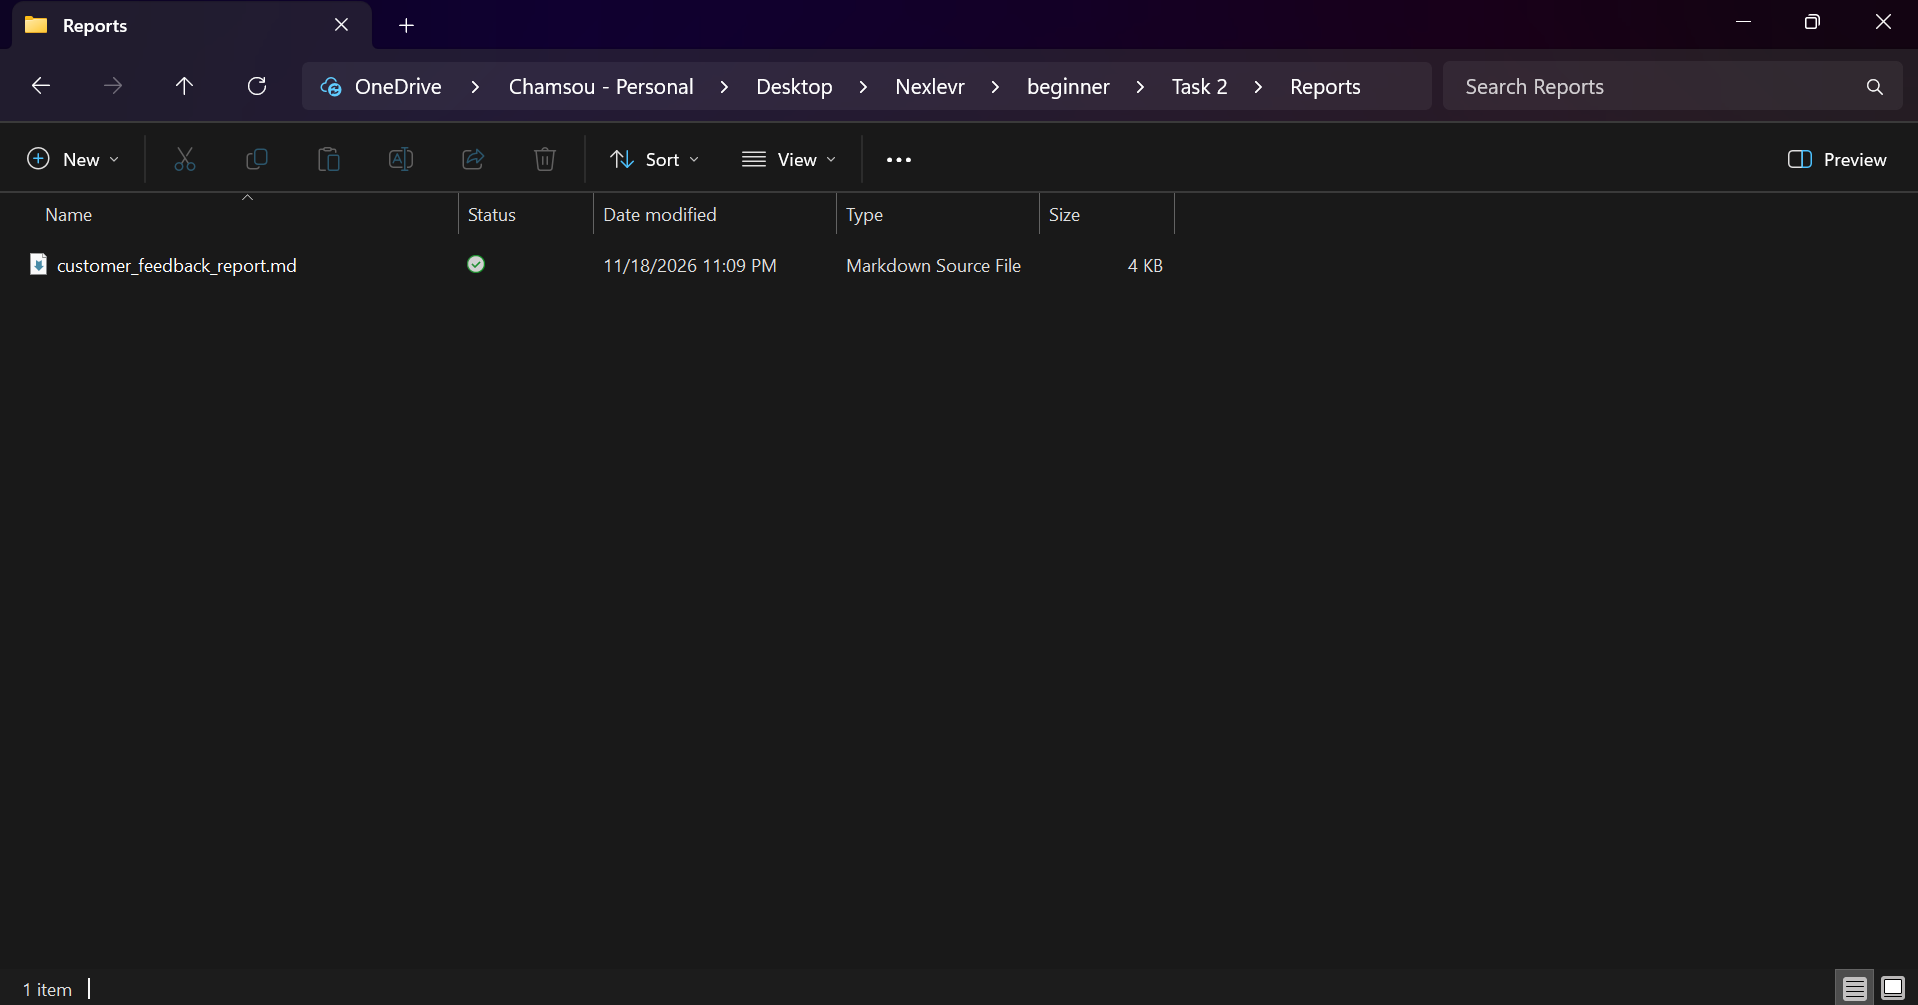
\includegraphics[width=\linewidth,height=5cm,keepaspectratio]{screenshot52.png}
		\end{minipage}
		
		\caption{Project directory showing the input and output folders.}
	\end{figure}
	
\end{document}
